\documentclass{article}

% these packages let you do math
\usepackage{amsmath}
\usepackage{amssymb}

% we need these packages for fancy R tables
\usepackage{booktabs}
\usepackage{float}
\usepackage{colortbl}
\usepackage{xcolor}

% these packages play with the spacing/margins of the document. Uncomment the commands on lines 16 and 17 to see what they do.
\usepackage{a4wide}
\usepackage{setspace}
\usepackage{geometry}
\usepackage{parskip}
%\doublespacing
%\geometry{margin=1.5in}

% this package helps us with including images. Setting the graphics path makes it easier to refer to things in the \includegraphics command.
\usepackage{graphicx}
\graphicspath{ {../figures/} }

% make some hyperlinks using the \href command
\usepackage{hyperref}
\hypersetup{
    colorlinks=true,
    linkcolor=black,
    urlcolor=blue
}

% set the author, title, and date of the document. \maketitle adds it to the document.
\author{Nathan Fraser}
\title{Hidden Curriculum Writeup}
\date{February 14th, 2022}

\begin{document}
\maketitle

\section{Explaining the relationship between incarceration, race and gender}

This dataset deals with youth in 2002, including information about their race, gender, age, and number of incarcerations. The bar graph sumarizes the data. In the bar graph it is shown that the mean number of incarcerations per person in 2002 were substantially higher for black people than for any other race. An interesting element of the bar graph is that mixed race non-hispanic males had no incarcerations in 2002. This is somewhat surprising; however, this may come from the face that mixed race males may genrally identify as being one race or another, not as 'mixed.' Another possibility is that these results occured by chance. There are few mixed race non-hispanic males in the data set and it is possible that purely by chance none of the few were incarcerated, despite a higher incarceration rate in the general population.


\begin{figure}[H]
    \begin{center}
        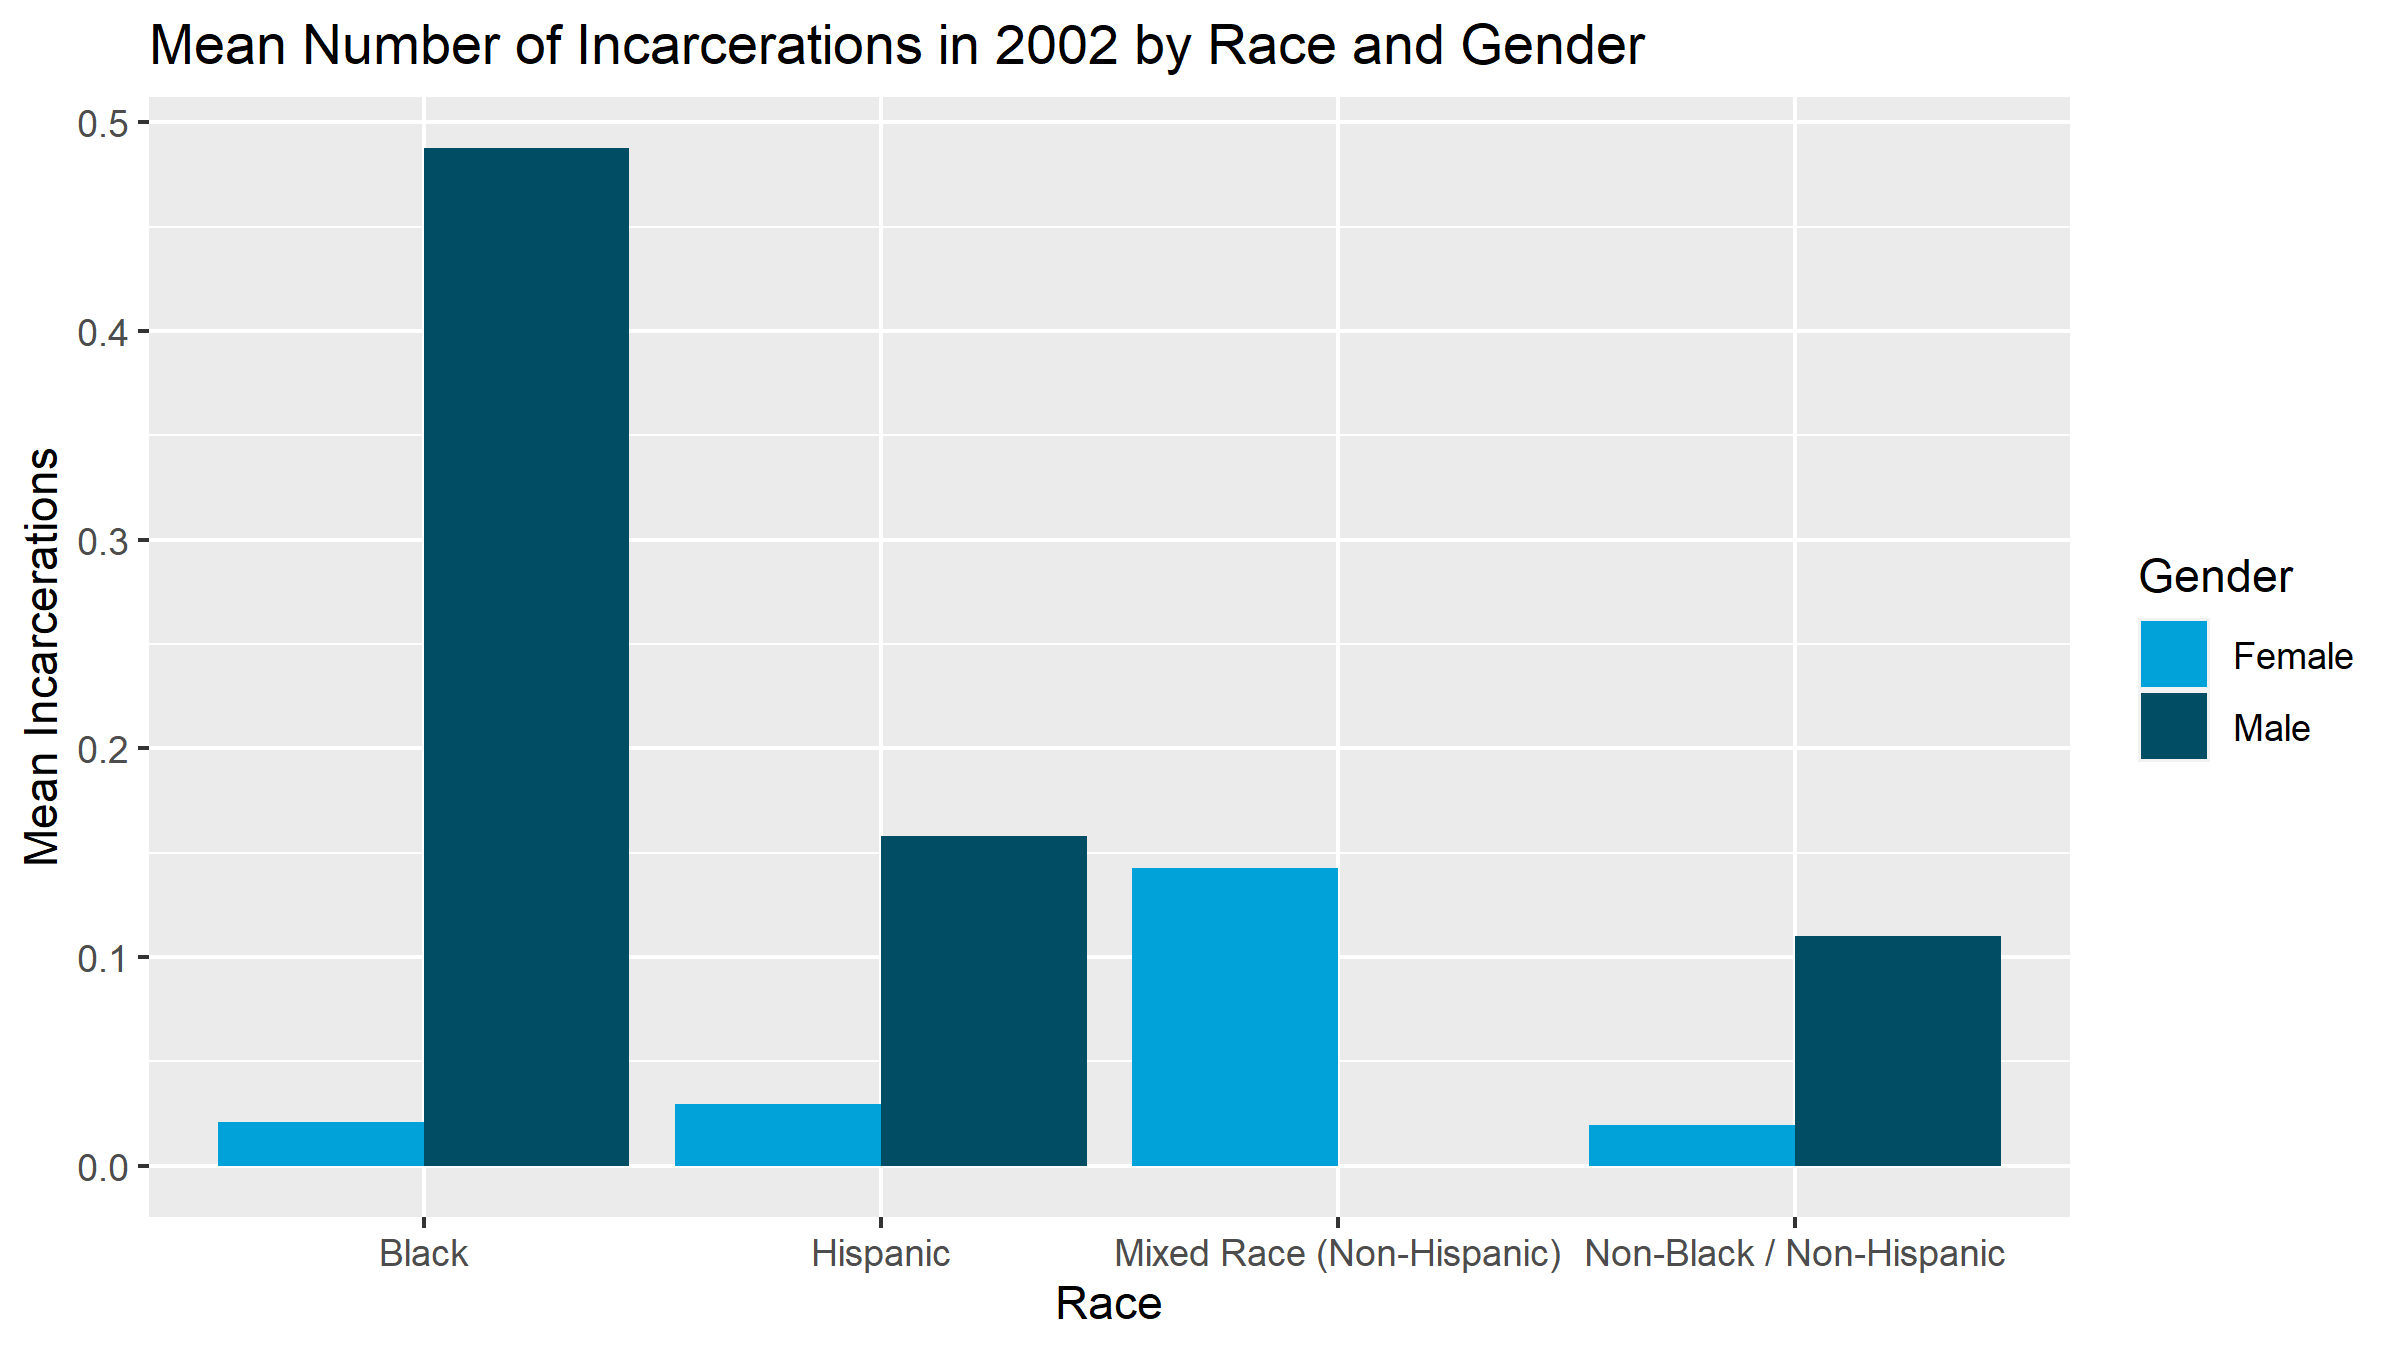
\includegraphics[width=.85\textwidth]{incarceration_by_racegender}
    \end{center}
    \caption{Mean Number of Incarcerations in 2002 by Race and Gender}
    \label{fig:graph}
\end{figure}


The following table provides the same information as the bar graph, just in numeric istead of visual format. Again, one can observe that the mean incarcerations for black males is much higher than for any other group at .4876712, more than double the second highest group (hispanic males) at .1579509. Also, we see that incarcerations for mixed race non-hispaic men is truly zero in our dataset, likely for the reasons discussed above.

\begin{table}[H]

\caption{\label{tab:tab:summarystats}Mean incarcerations in 2002 by Race and Gender}
\centering
\begin{tabular}[t]{lrrrr}
\toprule
Gender & Black & Hispanic & Mixed Race Non Hispanic & Non Black Non Hispanic\\
\midrule
\cellcolor{gray!6}{Female} & \cellcolor{gray!6}{0.0211268} & \cellcolor{gray!6}{0.0298013} & \cellcolor{gray!6}{0.1428571} & \cellcolor{gray!6}{0.0193192}\\
Male & 0.4876712 & 0.1579509 & 0.0000000 & 0.1099476\\
\bottomrule
\end{tabular}
\end{table}


The last table to examine is the regression output. In this regression, incarcerations is regressed on the race and gender dummies. The ommited categories are black and female, leading the interpretation of the coefficients to be in relataion to a black female baseline. We see negative coefficients on hispanic, mixed race, and non-black/non-hispanic suggesting that being those races is associated with a reduction in expected mean incarcerations per person. While the coefficient on male is positive, suggesting that being a black male, as opposed to black female, is associated with substantially more incarcerations. The R-Square is very low, .015, showing that the variance in these data are quite poorly explained by the variables in our regression. Additionally, the data here do not control for the myriad other factors, such as income, that could be associated with both race and number of incarcerations meaning we cannot establish causation.


% Table created by stargazer v.5.2.2 by Marek Hlavac, Harvard University. E-mail: hlavac at fas.harvard.edu
% Date and time: lu., feb. 14, 2022 - 14:19:59
\begin{table}[!htbp] \centering 
  \caption{Regression Output. Omitted category is Black Females.} 
  \label{tab:regression} 
\begin{tabular}{@{\extracolsep{5pt}}lc} 
\\[-1.8ex]\hline 
\hline \\[-1.8ex] 
 & \multicolumn{1}{c}{\textit{Dependent variable:}} \\ 
\cline{2-2} 
\\[-1.8ex] & Incarcerations in 2002 \\ 
\hline \\[-1.8ex] 
 Hispanic & $-$0.159$^{***}$ \\ 
  & (0.038) \\ 
  & \\ 
 Mixed Race (Non-Hispanic) & $-$0.174$^{**}$ \\ 
  & (0.083) \\ 
  & \\ 
 Non-Black / Non-Hispanic & $-$0.189$^{***}$ \\ 
  & (0.035) \\ 
  & \\ 
 Male & 0.194$^{***}$ \\ 
  & (0.022) \\ 
  & \\ 
 Constant & 0.155$^{***}$ \\ 
  & (0.026) \\ 
  & \\ 
\hline \\[-1.8ex] 
Observations & 8,621 \\ 
R$^{2}$ & 0.015 \\ 
Adjusted R$^{2}$ & 0.014 \\ 
Residual Std. Error & 1.019 (df = 8616) \\ 
F Statistic & 32.033$^{***}$ (df = 4; 8616) \\ 
\hline 
\hline \\[-1.8ex] 
\textit{Note:}  & \multicolumn{1}{r}{$^{*}$p$<$0.1; $^{**}$p$<$0.05; $^{***}$p$<$0.01} \\ 
\end{tabular} 
\end{table} 


\end{document}
